% preamble and style file for M&R lecture slides
\documentclass[11.5pt,sans,english]{beamer}

\usetheme{EastLansing}
\usecolortheme{lily}

\usepackage[most]{tcolorbox}

\usepackage{verbatim}
%\usepackage{ulem}
%\usepackage{fontawesome}
%\usepackage{tikz}
%\usepackage{pifont}
%\usepackage{tabularx}
\usepackage{array,booktabs,xcolor,colortbl,multirow,rotating,amssymb}
%\usepackage{amsmath}
% \usepackage{vwcol}
% \usepackage[T1]{fontenc}

  
\newcommand\vect[1]{\underline{\mathbf{#1}}}
\newcommand\unitvect[1]{\hat{\boldsymbol{#1}}}
%\newcommand\hatdot[1] { \hat{ \dot{ \boldsymbol{#1} } } }

\newtcbox
{\keyc}{on line,arc=2pt, colback=yellow!30!white, colframe=yellow!30!black, before upper={\rule[-3pt]{0pt}{10pt} },boxrule=1pt,boxsep=0pt,left=6pt,right=6pt,top=2pt,bottom=2pt,}

\newtcbox
{\keyb}{on line,arc=1pt, colback=blue!30!white, colframe=blue!30!black, before upper={\rule[-3pt]{0pt}{10pt} },boxrule=1pt,boxsep=0pt,left=6pt,right=6pt,top=2pt,bottom=2pt,}

\newtcbox
{\keyl}{on line,arc=1pt, colback=pink!30!white, colframe=blue!30!black, before upper={\rule[-3pt]{0pt}{10pt} },boxrule=1pt,boxsep=0pt,left=6pt,right=6pt,top=2pt,bottom=2pt,}

\newtcbox
{\keyw}{on line,arc=1pt, colback=red!30!white, colframe=blue!30!black, before upper={\rule[-3pt]{0pt}{10pt} },boxrule=1pt,boxsep=0pt,left=6pt,right=6pt,top=2pt,bottom=2pt,}

\newtcbox
{\keya}{on line,arc=1pt, colback=purple!30!white, colframe=blue!30!black, before upper={\rule[-3pt]{0pt}{10pt} },boxrule=1pt,boxsep=0pt,left=6pt,right=6pt,top=2pt,bottom=2pt,}

\newtcbox[auto counter,number within=section]
{keyf}
{
enhanced,
on line,
  boxsep=0pt,
  left=6pt,right=6pt,top=2pt,bottom=2pt,
  arc=5pt,
  boxrule=1pt,
  rightrule=38pt,
colback=green!10!white, 
colframe=green!50!black, 
title=\thetcbcounter,
detach title,
overlay unbroken and first ={
    \node[%rotate=90,
          %minimum width=1cm,
          anchor=south,
          font=\sffamily\bfseries\tiny,
          %yshift=-10pt,
          yshift=-5pt,
          xshift=-20pt,
          white]
    at (frame.east) {\thetcbcounter};
  }
}


\usepackage{xcolor}

%\usepackage{hyperref}
%\hypersetup{
%  pdfauthor={Lily Asquith},
%  urlcolor=blue,
%  colorlinks=true,
%  linkcolor=blue,
%  bookmarks=true
%}

%---------------------------------------------%
%              LILY'S COLOURS           %
%---------------------------------------------%
\definecolor{Wash}{RGB}{204,204,204}
%\definecolor{Pinky}{RGB}{254,200,254}%violet
\definecolor{Pinky}{RGB}{219,	240,	253}%violet
\definecolor{Bluey}{RGB}{0,190,255}%deep sky blue
\definecolor{DarkGrey}{RGB}{28,66,137}%dar grey
\definecolor{SussexWhite}{RGB}{253,255,254}%dar grey
\definecolor{LightGray}{RGB}{184,184,255}
\definecolor{YesGreen}{RGB}{0,128,0}
\definecolor{NoRed}{RGB}{250,0,0}



\definecolor{myred}{RGB}{255,153,153}
\definecolor{myorange}{RGB}{255,204,153}
\definecolor{myyellow}{RGB}{255,255,153}
\definecolor{mygreen}{RGB}{153,255,153}
\definecolor{mycyan}{RGB}{153,255,255}
\definecolor{myblue}{RGB}{153,204,255}
\definecolor{myviolet}{RGB}{153,153,255}
\definecolor{mypurple}{RGB}{204,153,255}
\definecolor{mypink}{RGB}{255,204,255}
\definecolor{mycoral}{RGB}{255,153,204}

%-----------------------------------------------------%
%              LILY'S COLUMN TYPES          %
%-----------------------------------------------------%
\newcolumntype{a}{>{\raggedright\arraybackslash}l}	
\newcolumntype{q}{>{\raggedright\arraybackslash}m{8cm}} 

%--------------------------------------------%
%              LILY'S SYMBOLS          %
%--------------------------------------------%
\newcommand{\dfinger}{\large{\textcolor{black}{\ding{43}}}\scriptsize}
\newcommand{\dstar}{\large{\textcolor{black}{\ding{76}}}\scriptsize}
\newcommand{\dwrite}{\large{\textcolor{black}{\ding{45}}}\scriptsize}
\newcommand{\ddiamond}{\small{\textcolor{DarkGrey}{\ding{117}}}\scriptsize}
\newcommand{\ddiamondwhite}{\small{\textcolor{SussexWhite}{\ding{117}}}\scriptsize}
\newcommand{\experiment}{\small{\textcolor{magenta}{\faCogs }}\scriptsize}
\newcommand{\watchit}{\textcolor{blue}{ \faYoutube}}


\makeatletter
\newcommand\notsotiny{\@setfontsize\notsotiny{6.5}{7.5}}
\makeatother


% 
\title[ Mechanics \& Relativity]{Mechanics \& Relativity}
%\subtitle{\textbf{Topic 1: Kinematics }}
\author[Dr Lily Asquith (Lily)]{ Dr Lily Asquith (Lily)}
\date[28-30 September 2021]{28-30 September 2021 (Week 1)}
\logo{

\includegraphics[width=1.5cm]{../../utils/uslogo.jpg}
}


\begin{document}


\begin{frame}
\titlepage
\end{frame} 

 %-----------------------------------------------------------%
 % 1 Kinematics                                                 %
 %-----------------------------------------------------------%
\section{M\&R 1: Kinematics}
\begin{frame}
\frametitle{Kinematics} 
\normalsize

This week's topics:\\[3ex]

\begin{itemize}
\item[1.1] Displacement, Velocity \& Acceleration\\[3ex]
\item[1.2] Equations of motion (SUVAT)\\[3ex]
\item[1.3] Reading graphs\\[3ex]
\end{itemize}
\end{frame} 
 
 %-----------------------------------------------------------%
 % LECTURE 1
 %-----------------------------------------------------------%
 
 \subsection{Displacement, Velocity \& Acceleration }

%  
\begin{frame}{Notation}
$s$ : for position (or sometimes $x$, or $y$, or $r$...)\\
%$\vect{s}$ or $\vec{s}$ : for linear displacement with a direction\\
$u$ : for (magnitude of) initial velocity (aka initial speed)\\
$v$ : for (magnitude of) velocity (aka speed)\\
%$\vect{v}$ or $\vec{v}$ : for speed with a direction (velocity)\\
$a$ : for (magnitude of) acceleration\\
%$\vect{a}$ or $\vec{a}$ : for acceleration with a direction\\
$t$ : for time (\textcolor{blue}{is time a vector?})\\[1ex]
$\Delta$ : means \textit{`change in'} \\[1ex]
$\delta$ or $d$ : means \textit{`teeny weeny change in'} \\[1ex]

Standard units of displacement in space and time are metres and seconds, unless otherwise stated.\\

\end{frame}
 
% 
\begin{frame}{Displacement}
\small
To begin to talk about where something is, let alone where it is headed, we need three things:
\begin{itemize}
\item[1]  A coordinate system, $eg$ cartesian coordinates (x, y, z).
\item[2]  A reference point: \textbf{the origin}.\\[1ex]
\item[3]  A positive direction.\\[1ex]
\end{itemize}

\begin{center}
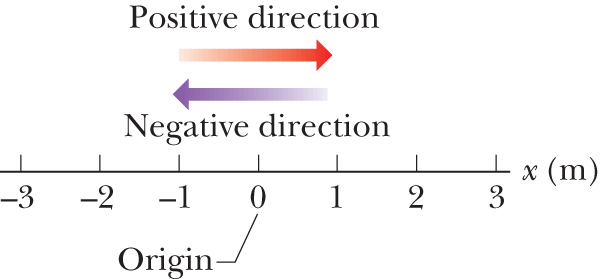
\includegraphics[scale=0.8]{1.png}
\end{center}

We can then define the displacement as \textbf{ the change in position:} \\[1ex]

\keyf{ $\Delta s = s_{f} - s_{i}$}  

\end{frame}
 
 \begin{frame}{Poll everywhere checkpoint }
 Here are three pairs of initial and final positions: [$s_i, s_f$] along an x axis. Which pairs give a \textit{negative displacement $\Delta s$}?\\[1ex]
 (a) [-3 m, +5 m]\\ 
 (b) [-3 m, -7 m]\\
 (c) [7 m, -3 m]\\[3ex]

\fbox{\begin{minipage}{\textwidth}
Use your phone to go to: \textcolor{blue}{pollev.com/ilovephysics} and select the option:\\
 A :  a \& b give negative displacements\\
 B :  a \& c   \\
 C :  b \& c 
 \end{minipage}}
 \vspace{0.5cm}
 
 Don't panic, these polls are always anonymous!
 
 
 \end{frame}
 
 % 
\begin{frame}{Displacement}
An object may be motionless in space, but it will always move through time.\\[2ex]
\centering
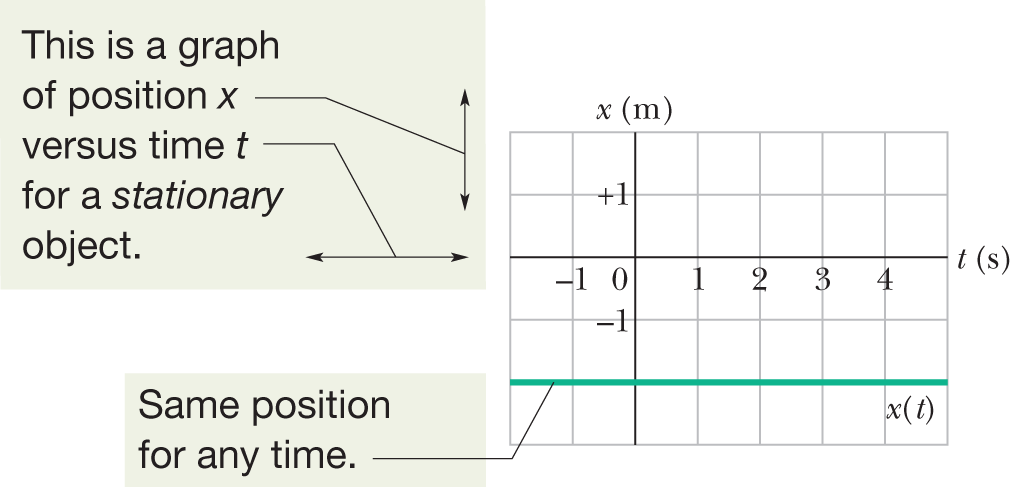
\includegraphics[scale=1.]{2.png}
\end{frame}


% 
\begin{frame}{Average velocity}
To find the average velocity, we divide the total distance by the total time.\\[2ex] 
\centering
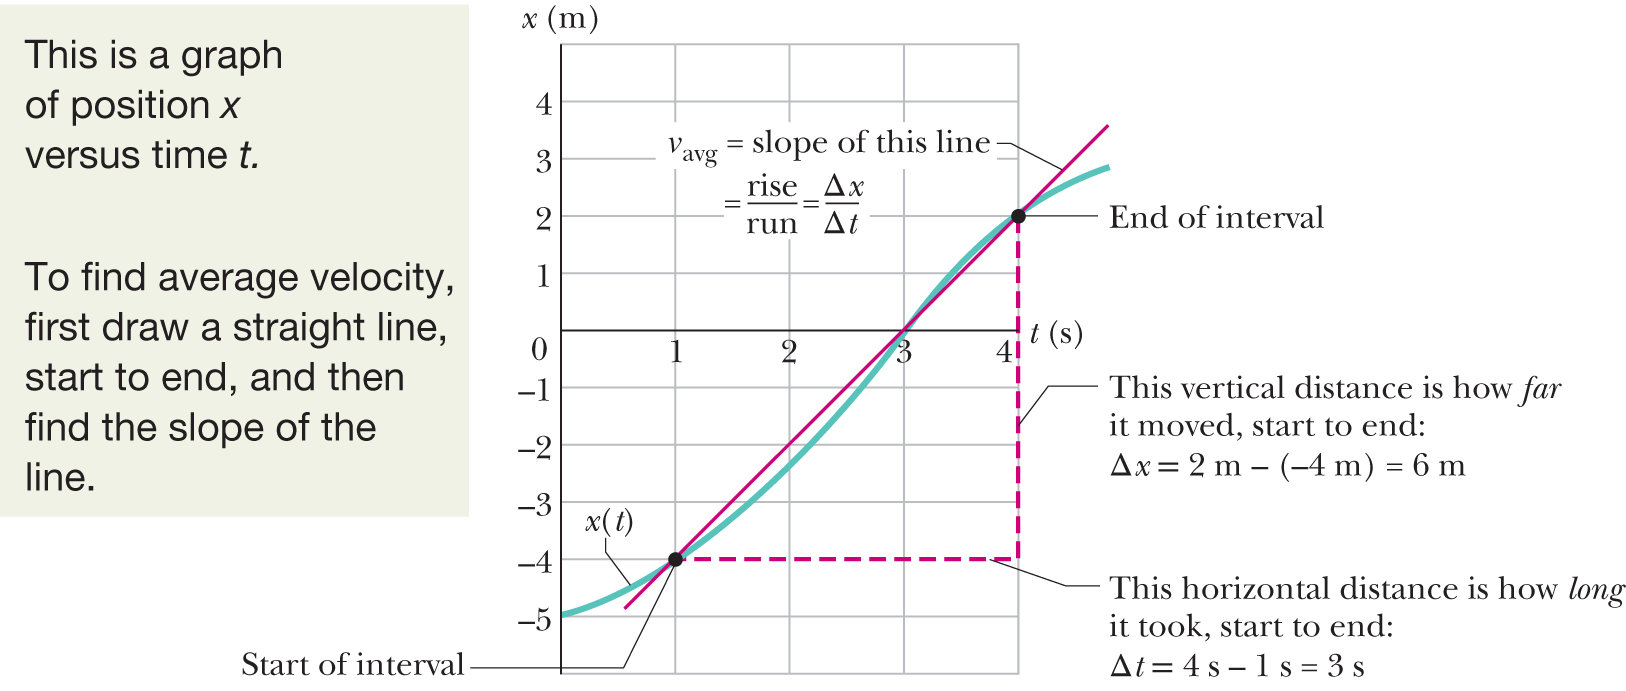
\includegraphics[scale=0.8]{3.png}
\end{frame}


%   
\begin{frame}{Solving a problem of this sort}
\small
You drive along a straight road for 8.4 km at 70 km/h, at which point your car runs out of petrol and stops. Over the next 30 min, you walk another 2.0 km along the road to a petrol station.\\[1ex]
\textit{What are your overall displacement, time taken, and average speed from the beginning of your drive to your arrival at the station?}\\[1ex]

\vspace{5cm}
\end{frame}

 
 %  
\begin{frame}{Instantaneous velocity}

We can define the velocity (and acceleration) either as average or as instantaneous.\\[2ex]

The average velocity and acceleration over a period of time given by $\Delta t$ is: \\[2ex]
\keyf{$\vect{v}_{avg} = \frac{\Delta \vect{s} }{\Delta t} $; \;\; $\vect{a}_{avg} = \frac{\Delta \vect{v} }{\Delta t} $} \\[2ex]

The instantaneous velocity and acceleration  at an exact moment in time is: \\[2ex]
\keyf{$\vect{v} = \frac{\delta  }{\delta t} \vect{s}$; \;\; $\vect{a} = \frac{\delta  }{\delta t} \vect{v}= \frac{\delta^2  }{\delta t^2} \vect{s}$} \\[1ex]
\end{frame}



%  
\begin{frame}{A bit more notation / reminder of calculus...}

$\frac{d s }{d t} $: the differential of position With Respect To (wrt) time.\\[1ex]
$\frac{d^2 s }{d t^2} $ : the second differential of position wrt time.\\[3ex]

Example \& Notation: \\[10ex]






\end{frame}

 
  \begin{frame}{Checkpoint }
  \small
The following equations give the position $x(t)$ of a particle in four situations (in each equation, $x$ is in meters, $t$ is in seconds, and $t > 0$):\\[2ex]

 (1) $x = 3t - 2$\\[1ex]
 (2) $x = -4t^2 - 2$\\[1ex]
 (3) $x = \frac{2}{t^2}$\\[1ex]
 (4) $x = -2$ \\[3ex]
 
%\fbox{\begin{minipage}{\textwidth}
%Use your phone to go to: \textcolor{blue}{pollev.com/ilovephysics}
 (a) In which situation(s) is the velocity v of the particle constant? \\[2ex]
 (b) In which is v in the negative x direction?\\
%\end{minipage}}
\vspace{2cm}
 
 
 \end{frame}
 
 %  
\begin{frame}{Acceleration}
\small
Acceleration usually means `speeding up' in normal conversation. In physics it also means `slowing down'.\\[1ex]

If something has a changing speed, then its acceleration is non-zero\\[1ex]

Which of these positions as a function of time correspond to constant acceleration?\\[1ex]
$x = 4t^3 - 55$:\\[1ex]
$x = 4t^2 - 55$:\\[1ex]
$x = 4t - 55$:\\[1ex]
$x = 4/t - 55$:\\[1ex]
$x = 4/t^2 - 55$:\\[1ex]
%$x = 4/t^3 - 55$:\\[1ex]
\end{frame}


\begin{frame}{Before next lecture}

Retry the pre-lecture quiz 1.1  Velocity and Acceleration, if you like.\\[2ex]
Attempt the pre-lecture quiz for 1.2  Equations of Motion.\\[2ex]
See you tomorrow morning for lecture 1.2\\

\end{frame}



 
\end{document}